\documentclass[aspectratio=169,10pt]{beamer}
\usepackage{issa}  % place issa.sty in the same folder
\definecolor{AccentCol}{HTML}{6D4C41}
\renewcommand{\lecnum}{6}
\title{AI \& Machine Learning in Warfare}

\tikzset{
 neu/.style={circle,draw=ISSAnavy,line width=0.6pt,minimum size=0.8cm,inner sep=0pt,align=center,font=\fontsize{6.5}{7.5}\selectfont,fill=white},
 inp/.style={neu,fill=ISSAgrn!12,draw=ISSAgrn},
 hid/.style={neu,fill=AccentCol!14,draw=AccentCol},
 outp/.style={neu,fill=AccentCol!35,draw=AccentCol},
 wl/.style={font=\fontsize{5.8}{6.8}\selectfont,fill=ISSAvlight,inner sep=0.6pt},
 cls0/.style={circle,draw=ISSAblue,fill=ISSAblue!30,inner sep=2.2pt},
 cls1/.style={rectangle,draw=ISSAred,fill=ISSAred!35,inner sep=2.6pt}}

% unit-square scatter with four XOR-style corners: \xorpts{c00}{c01}{c10}{c11}
\newcommand{\cornerplot}[5]{%
\begin{tikzpicture}[scale=2.0]
\draw[ISSAgrey!40] (0,0) grid[step=0.5] (1,1);
\draw[-{Stealth[length=3pt]},ISSAdark] (-0.1,0)--(1.25,0) node[right,font=\scriptsize]{$x_1$};
\draw[-{Stealth[length=3pt]},ISSAdark] (0,-0.1)--(0,1.25) node[above,font=\scriptsize]{$x_2$};
\node[#1] at (0,0) {}; \node[#2] at (0,1) {}; \node[#3] at (1,0) {}; \node[#4] at (1,1) {};
\node[font=\tiny,below left] at (0,0) {0}; \node[font=\tiny,below] at (1,0) {1}; \node[font=\tiny,left] at (0,1) {1};
#5
\end{tikzpicture}}


% ---------- shared figures ----------
\newcommand{\netfig}{%
\begin{tikzpicture}[x=1cm,y=1cm,
 neu/.style={circle,draw=ISSAnavy,line width=0.6pt,minimum size=0.95cm,inner sep=0pt,align=center,font=\fontsize{6.5}{7.5}\selectfont},
 inp/.style={neu,fill=ISSAgrn!12,draw=ISSAgrn},
 hid/.style={neu,fill=AccentCol!12,draw=AccentCol},
 outn/.style={neu,fill=AccentCol!30,draw=AccentCol},
 wl/.style={font=\fontsize{5.6}{6.5}\selectfont,fill=ISSAvlight,inner sep=0.6pt},
 bx/.style={nd,font=\fontsize{5.5}{6.5}\selectfont,minimum height=0.32cm,inner sep=1.5pt}]
\node[inp] (x1) at (0,1.15) {$x_1$\\1.0};
\node[inp] (x2) at (0,-1.15) {$x_2$\\0.5};
\node[hid] (h1) at (3.4,1.15) {$z^{(1)}_1|a^{(1)}_1$\\$\sigma$};
\node[hid] (h2) at (3.4,-1.15) {$z^{(1)}_2|a^{(1)}_2$\\$\sigma$};
\node[outn] (o) at (6.6,0) {$z^{(2)}|a^{(2)}$\\$\sigma$};
\node[ndR,font=\fontsize{6}{7}\selectfont] (L) at (8.7,0) {BCE\\$L(a^{(2)},y)$};
\node[bx] (b11) at (3.4,2.25) {$b^{(1)}_1=0$};
\node[bx] (b12) at (3.4,-2.25) {$b^{(1)}_2=0$};
\node[bx] (b2) at (6.6,1.2) {$b^{(2)}=0.1$};
\draw[arr] (x1)--node[wl,above=0.5pt]{$w^{(1)}_{11}=0.4$}(h1);
\draw[arr] (x2)--node[wl,below=0.5pt]{$w^{(1)}_{22}=0.6$}(h2);
\draw[arr] (x2)--node[wl,pos=0.72,sloped,above=0.5pt]{$w^{(1)}_{12}=-0.2$}(h1);
\draw[arr] (x1)--node[wl,pos=0.72,sloped,below=0.5pt]{$w^{(1)}_{21}=0.3$}(h2);
\draw[arr] (h1)--node[wl,above,sloped]{$w^{(2)}_1=0.7$}(o);
\draw[arr] (h2)--node[wl,below,sloped]{$w^{(2)}_2=-0.5$}(o);
\draw[arr] (o)--(L);
\draw[arr,dashed,ISSAgrey] (b11)--(h1);
\draw[arr,dashed,ISSAgrey] (b12)--(h2);
\draw[arr,dashed,ISSAgrey] (b2)--(o);
\end{tikzpicture}}

\begin{document}
\titleslide{6}{Neural Networks:\\Hidden Layers \& Backpropagation}{Part 1: why hidden layers --- one neuron's straight line, the XOR wall, non-linear activations and learned feature maps\\Part 2: backpropagation by hand --- one forward and one backward pass through a 2--2--1 sigmoid network}


%====================================================================
\sect{1. Overview}
\begin{frame}{Learning Objectives \& Session Structure}
\begin{columns}[T]
\column{0.55\textwidth}
\begin{cbox}{By the end of this lecture you will be able to}
\begin{te}
\item Show that one neuron draws one straight boundary, and prove it cannot compute XOR
\item Show that wide-but-linear layers, or stacked linear layers, add no power
\item Solve XOR by hand with one ReLU hidden layer; explain hidden layers as \emph{learned feature maps}
\item State the universal approximation theorem, its fine print, and why depth still matters
\item Run a full forward pass $z^{(1)}\!\to a^{(1)}\!\to z^{(2)}\!\to a^{(2)}\!\to L$ in a 2--2--1 sigmoid network
\item Derive $\delta^{(2)}=a^{(2)}-y$ and back-propagate it with the chain rule
\item Compute every gradient and one gradient-descent update, and check its effect
\end{te}
\end{cbox}
\column{0.42\textwidth}
\begin{cbox}[ISSAnavy]{Session Structure (45 min)}
\begin{tl}
\item \textbf{5 min} --- Opening Q\&A: recap of Lectures 1--5
\item \textbf{13 min} --- \textbf{Part 1, Why hidden layers?} One neuron, the XOR wall, non-linearity, XOR solved, feature maps
\item \textbf{17 min} --- \textbf{Part 2, Backpropagation by hand:} set-up, forward pass, backward pass, update and check
\item \textbf{10 min} --- Auto-quiz (15 questions)
\end{tl}
\end{cbox}
\begin{ibox}\scriptsize\textbf{Where this leads:} every network in the rest of the course --- the CNN (L7), the transformer (L8--L9), the DQN and PPO agents (L10--L11) --- has hidden layers with non-linear activations, and every one is trained by the backpropagation of Part~2.\end{ibox}
\end{columns}
\end{frame}


\begin{frame}{The Story in One Slide}
\figc{3.1cm}{%
\begin{tikzpicture}[node distance=0.45cm]
\node[ndR,minimum width=2.6cm,minimum height=1.25cm] (a) {\textbf{One neuron}\\one straight line\\\emph{fails on XOR}};
\node[ndR,right=of a,minimum width=2.6cm,minimum height=1.25cm] (b) {\textbf{One wide layer}\\many separate lines\\\emph{still cannot combine}};
\node[ndR,right=of b,minimum width=2.6cm,minimum height=1.25cm] (c) {\textbf{Linear layers stacked}\\collapse into one\\\emph{no gain}};
\node[ndG,right=of c,minimum width=2.6cm,minimum height=1.25cm] (d) {\textbf{Hidden layer +}\\\textbf{non-linearity}\\\emph{bends space: XOR solved}};
\node[ndC,right=of d,minimum width=2.6cm,minimum height=1.25cm] (e) {\textbf{Many hidden layers}\\features of features\\\emph{feature maps}};
\draw[arr] (a)--(b); \draw[arr] (b)--(c); \draw[arr] (c)--(d); \draw[arr] (d)--(e);
\end{tikzpicture}}
\vspace{3pt}
\begin{columns}[T]
\column{0.32\textwidth}
\begin{cbox}{The limitation}\scriptsize A neuron computes a weighted sum, so its boundary is a straight line (a plane in higher dimensions).\end{cbox}
\column{0.32\textwidth}
\begin{cbox}{The fix}\scriptsize Put a \emph{non-linear} activation between layers; the hidden layer re-maps the data into new coordinates.\end{cbox}
\column{0.32\textwidth}
\begin{cbox}{The bonus}\scriptsize Those new coordinates are \emph{features} the network invents for itself --- no manual feature engineering.\end{cbox}
\end{columns}
\end{frame}

%====================================================================
\sect{2. One Neuron}
\begin{frame}{A Single Neuron Draws a Straight Line}
\begin{columns}[T]
\column{0.48\textwidth}
\figc{2.6cm}{%
\begin{tikzpicture}[x=1cm,y=1cm]
\node[inp] (x1) at (0,0.7) {$x_1$}; \node[inp] (x2) at (0,-0.7) {$x_2$};
\node[outp,minimum size=1.1cm] (n) at (2.6,0) {$\Sigma\,|\,f$};
\node[nd,font=\scriptsize] (b) at (2.6,1.25) {$b$};
\draw[arr] (x1)--node[wl,above]{$w_1$}(n); \draw[arr] (x2)--node[wl,below]{$w_2$}(n); \draw[arr] (b)--(n);
\draw[arr] (n)--(4.0,0) node[right,font=\scriptsize]{$\hat y$};
\end{tikzpicture}}
\begin{fbx}{Decision boundary}
$w_1x_1+w_2x_2+b=0\quad\Longleftrightarrow\quad x_2=-\dfrac{w_1}{w_2}x_1-\dfrac{b}{w_2}$
\end{fbx}
\begin{cbox}{Whatever the activation}\scriptsize Step, sigmoid or ReLU are all \emph{monotonic} in $z=w\cdot x+b$, so ``output above threshold'' is the same as ``$z$ above some constant''. The boundary is always a straight line --- in $d$ dimensions, a flat hyperplane.\end{cbox}
\column{0.49\textwidth}
\figc{4.6cm}{%
\begin{tikzpicture}
\begin{axis}[width=6.6cm,height=5.6cm,xmin=0,xmax=1,ymin=0,ymax=1,grid=major,grid style={ISSAgrey!20},xlabel={$x_1$},ylabel={$x_2$},title={One neuron: $z=2x_1+x_2-1.2$}]
\addplot[fill=ISSAred!12,draw=none] coordinates{(0.6,0)(1,0)(1,1)(0.1,1)} \closedcycle;
\addplot[AccentCol,line width=1.4pt,domain=0.1:0.6]{1.2-2*x};
\node[font=\scriptsize,text=ISSAred] at (axis cs:0.78,0.62) {$z>0$: class 1};
\node[font=\scriptsize,text=ISSAblue] at (axis cs:0.2,0.25) {$z<0$: class 0};
\node[font=\scriptsize,text=AccentCol,rotate=-55] at (axis cs:0.42,0.48) {$z=0$};
\end{axis}
\end{tikzpicture}}
\begin{ibox}\scriptsize Training a single neuron only \emph{moves and rotates} this line. It can never bend it.\end{ibox}
\end{columns}
\end{frame}

\begin{frame}{What One Neuron Can Do: AND and OR}
\begin{columns}[T]
\column{0.32\textwidth}
\centering
\figc{3.2cm}{\cornerplot{cls0}{cls0}{cls0}{cls1}{\draw[AccentCol,line width=1.3pt] (0.5,1.15)--(1.15,0.5);}}
\begin{cbox}{AND: $w=(1,1),\ b=-1.5$}\scriptsize
\renewcommand{\arraystretch}{1.05}\centering
\begin{tabular}{ccrc}
$x_1$&$x_2$&$z$&$\hat y$\\\midrule
0&0&$-1.5$&0\\0&1&$-0.5$&0\\1&0&$-0.5$&0\\1&1&$0.5$&\textbf{1}
\end{tabular}
\end{cbox}
\column{0.32\textwidth}
\centering
\figc{3.2cm}{\cornerplot{cls0}{cls1}{cls1}{cls1}{\draw[AccentCol,line width=1.3pt] (-0.1,0.6)--(0.6,-0.1);}}
\begin{cbox}{OR: $w=(1,1),\ b=-0.5$}\scriptsize
\renewcommand{\arraystretch}{1.05}\centering
\begin{tabular}{ccrc}
$x_1$&$x_2$&$z$&$\hat y$\\\midrule
0&0&$-0.5$&0\\0&1&$0.5$&\textbf{1}\\1&0&$0.5$&\textbf{1}\\1&1&$1.5$&\textbf{1}
\end{tabular}
\end{cbox}
\column{0.32\textwidth}
\begin{cbox}[ISSAnavy]{Rule: step output}\scriptsize $\hat y=1$ if $z=w_1x_1+w_2x_2+b>0$, else 0. Both problems are \textbf{linearly separable}: one line puts all squares on one side and all circles on the other.\end{cbox}
\begin{ibox}\scriptsize Rosenblatt's perceptron (1958) learned exactly such lines, and it was hailed as the start of machine intelligence.\end{ibox}
\begin{rbox}\scriptsize Legend: \tikz\node[cls0]{}; = class 0, \ \tikz\node[cls1]{}; = class 1.\end{rbox}
\end{columns}
\end{frame}

\begin{frame}{The XOR Wall: A Problem No Single Neuron Can Solve}
\begin{columns}[T]
\column{0.34\textwidth}
\centering
\figc{3.4cm}{\cornerplot{cls0}{cls1}{cls1}{cls0}{\draw[ISSAred,dashed,line width=1pt] (-0.1,0.55)--(1.15,0.7); \node[font=\tiny,text=ISSAred] at (0.75,0.95) {any line fails};}}
\scriptsize XOR: output 1 when the inputs \emph{differ}. The squares sit on one diagonal, the circles on the other.
\column{0.63\textwidth}
\begin{cbox}{Proof by contradiction}
\scriptsize Suppose some $w_1,w_2,b$ worked (output 1 iff $z>0$). The four rows of the truth table demand:
\[
\begin{array}{lll}
(0,0)\to0: & b\le0 & (1)\\
(1,0)\to1: & w_1+b>0 & (2)\\
(0,1)\to1: & w_2+b>0 & (3)\\
(1,1)\to0: & w_1+w_2+b\le0 & (4)
\end{array}
\]
Add (2) and (3): $w_1+w_2+2b>0$, so $w_1+w_2+b>-b\ge0$ using (1). This contradicts (4). \hfill$\blacksquare$
\end{cbox}
\begin{wbox}\scriptsize\textbf{History:} Minsky and Papert's book \emph{Perceptrons} (1969) highlighted this limitation; it contributed to a long slump in neural-network research until multi-layer training (backpropagation) was popularised in 1986.\end{wbox}
\end{columns}
\end{frame}

\begin{frame}{XOR Is Not a Toy: Non-Separable Patterns in Real Data}
\begin{columns}[T]
\column{0.50\textwidth}
\figc{5.0cm}{%
\begin{tikzpicture}
\begin{axis}[width=7cm,height=5.8cm,xmin=0,xmax=1,ymin=0,ymax=1,grid=major,grid style={ISSAgrey!20},xlabel={normalised speed},ylabel={normalised altitude},title={Air tracks (synthetic, illustrative)},legend pos=outer north east,legend style={at={(0.5,-0.25)},anchor=north,legend columns=2}]
\addplot[only marks,mark=square*,mark size=1.6pt,ISSAred] coordinates{(0.88,0.27) (0.50,0.22) (0.83,0.16) (0.72,0.17) (0.73,0.13) (0.76,0.08) (0.56,0.16) (0.75,0.25) (0.68,0.17) (0.33,0.77) (0.20,0.77) (0.22,0.91) (0.39,0.70) (0.28,0.77) (0.16,0.90) (0.20,0.86) (0.28,0.81) (0.43,0.87)};
\addplot[only marks,mark=*,mark size=1.6pt,ISSAblue] coordinates{(0.02,0.21) (0.33,0.37) (0.11,0.30) (0.04,0.24) (0.25,0.34) (0.30,0.20) (0.17,0.12) (0.10,0.28) (0.22,0.28) (0.76,0.88) (0.69,0.58) (0.81,0.70) (0.51,0.88) (0.86,0.93) (0.83,0.56) (0.60,0.75) (0.79,0.84) (0.67,0.73)};
\legend{hostile,routine}
\node[font=\fontsize{5.5}{6.5}\selectfont,text=ISSAred] at (axis cs:0.78,0.36) {fast \& low};
\node[font=\fontsize{5.5}{6.5}\selectfont,text=ISSAred] at (axis cs:0.25,0.62) {slow \& high};
\node[font=\fontsize{5.5}{6.5}\selectfont,text=ISSAblue] at (axis cs:0.2,0.05) {slow \& low};
\node[font=\fontsize{5.5}{6.5}\selectfont,text=ISSAblue] at (axis cs:0.75,0.98) {fast \& high};
\end{axis}
\end{tikzpicture}}
\column{0.47\textwidth}
\begin{cbox}{An XOR-shaped threat picture (illustrative)}\scriptsize
\begin{tl}
\item \textbf{Fast \& low}: sea-skimming or cruise-missile profile --- hostile
\item \textbf{Slow \& high}: loitering surveillance platform --- hostile
\item \textbf{Slow \& low}: own helicopters --- routine
\item \textbf{Fast \& high}: airliners, own jets --- routine
\end{tl}
Neither speed nor altitude alone separates the classes; only their \emph{combination} does --- the XOR pattern.
\end{cbox}
\begin{wbox}\scriptsize A single neuron (logistic regression) on these two inputs can do little better than guessing the majority class.\end{wbox}
\begin{ibox}\scriptsize Other common non-separable shapes: a target inside a ring of clutter, interleaved spirals, ``either A or B but not both'' rules.\end{ibox}
\end{columns}
\end{frame}

%====================================================================
\sect{3. Wide Is Not Enough}
\begin{frame}{One Layer with Many Neurons Is Still Linear}
\begin{columns}[T]
\column{0.46\textwidth}
\figc{3.4cm}{%
\begin{tikzpicture}[x=1cm,y=1cm]
\node[inp] (x1) at (0,0.8) {$x_1$}; \node[inp] (x2) at (0,-0.8) {$x_2$};
\foreach \i/\y in {1/1.5,2/0.5,3/-0.5,4/-1.5}{\node[outp] (o\i) at (2.6,\y) {$\hat y_{\i}$}; \draw[arr] (x1)--(o\i); \draw[arr] (x2)--(o\i);}
\node[lab,anchor=west] at (3.1,0) {4 outputs = 4 independent lines};
\end{tikzpicture}}
\begin{fbx}{A single layer}
$\hat y_k=f\bigl(w_k\cdot x+b_k\bigr),\quad k=1,\dots,K$
\end{fbx}
\column{0.51\textwidth}
\begin{wbox}\scriptsize\textbf{No neuron sees another neuron's answer.} Each output draws its own line on the \emph{same raw inputs}; nothing combines them. For XOR, every one of the $K$ neurons faces the same impossibility proof.\end{wbox}
\begin{cbox}{Multi-class is also linear}\scriptsize With softmax over $K$ outputs (multinomial logistic regression), class $k$ wins where $w_k\cdot x+b_k$ is largest. The regions are separated by straight lines, and every region is \emph{convex} --- no class can occupy two opposite corners.\end{cbox}
\begin{ibox}\scriptsize Width alone adds more lines; it does not let the network \emph{reason with} those lines (``inside line 1 AND outside line 2''). That needs a second stage that takes the lines as its inputs --- a hidden layer.\end{ibox}
\end{columns}
\end{frame}

\begin{frame}{Stacking Linear Layers Collapses into One}
\begin{columns}[T]
\column{0.52\textwidth}
\begin{cbox}{The algebra}
\scriptsize Two layers with \emph{no} activation (identity $f$):
\[
\hat y=W_2\bigl(W_1x+b_1\bigr)+b_2=\underbrace{(W_2W_1)}_{W}\,x+\underbrace{(W_2b_1+b_2)}_{b}
\]
A product of matrices is just another matrix, so 2 --- or 100 --- linear layers equal \textbf{one} linear layer.
\end{cbox}
\begin{cbox}{Numerical check}
\scriptsize $W_1=\begin{pmatrix}1&2\\0&1\end{pmatrix},\ b_1=\begin{pmatrix}1\\0\end{pmatrix},\ W_2=(1\ \ -1),\ b_2=0.5$\\[3pt]
Collapsed: $W=W_2W_1=(1,\ 1)$, \ $b=W_2b_1+b_2=1.5$\\[3pt]
At $x=(1,1)$: \ two layers $\to h=(4,1)$, $\hat y=4-1+0.5=\hl{3.5}$;\ \ one layer $\to 1+1+1.5=\hl{3.5}$.\\
At $x=(2,-1)$: both give $\hl{2.5}$.
\end{cbox}
\column{0.45\textwidth}
\figc{2.8cm}{%
\begin{tikzpicture}[node distance=0.35cm]
\node[ndA] (x) {$x$}; \node[ndN,right=of x] (l1) {$W_1,b_1$}; \node[ndN,right=of l1] (l2) {$W_2,b_2$}; \node[ndA,right=of l2] (y) {$\hat y$};
\draw[arr] (x)--(l1); \draw[arr] (l1)--(l2); \draw[arr] (l2)--(y);
\node[ndA,below=0.8cm of x] (xx) {$x$}; \node[ndN,right=1.3cm of xx] (l) {$W,b$}; \node[ndA,below=0.8cm of y] (yy) {$\hat y$};
\draw[arr] (xx)--(l); \draw[arr] (l)--(yy);
\node[font=\Large,text=AccentCol] at ($(l1)!0.5!(l2)+(0,-0.85)$) {$\equiv$};
\end{tikzpicture}}
\begin{wbox}\scriptsize\textbf{Conclusion:} depth without non-linearity is an illusion. The hidden layer must \emph{bend} its output, or the network is still a single straight line.\end{wbox}
\begin{ibox}\scriptsize The same argument shows why every CNN conv layer and every Transformer feed-forward block is followed by a non-linear activation.\end{ibox}
\end{columns}
\end{frame}

%====================================================================
\sect{4. Non-Linearity}
\begin{frame}{Non-Linear Activation Functions}
\begin{columns}[T]
\column{0.50\textwidth}
\figc{4.8cm}{%
\begin{tikzpicture}
\begin{axis}[width=7cm,height=5.6cm,xmin=-3,xmax=3,ymin=-1.2,ymax=3,grid=major,grid style={ISSAgrey!20},xlabel={$z$},ylabel={$f(z)$},legend pos=north west,legend style={font=\fontsize{5.5}{6.5}\selectfont}]
\addplot[ISSAgrey,line width=1pt,const plot,domain=-3:3,samples=2] coordinates{(-3,0)(0,0)(0,1)(3,1)};
\addplot[ISSAblue,line width=1pt,domain=-3:3,samples=100]{1/(1+exp(-x))};
\addplot[ISSAgrn,line width=1pt,domain=-3:3,samples=100]{tanh(x)};
\addplot[AccentCol,line width=1.4pt,domain=-3:3,samples=100]{max(0,x)};
\legend{step,sigmoid,tanh,ReLU}
\end{axis}
\end{tikzpicture}}
\column{0.47\textwidth}
\centering\scriptsize\renewcommand{\arraystretch}{1.35}\setlength{\tabcolsep}{3pt}
\begin{tabular}{lll}
\toprule
\textbf{Name}&$f(z)$&\textbf{Notes}\\\midrule
Step&$1$ if $z>0$, else $0$&no usable gradient\\
Sigmoid&$1/(1+e^{-z})$&range $(0,1)$; $f'\le0.25$\\
Tanh&$\tanh z$&range $(-1,1)$\\
ReLU&$\max(0,z)$&default; $f'=1$ if $z>0$\\\bottomrule
\end{tabular}
\vspace{4pt}
\raggedright
\begin{cbox}{What a non-linearity must do}\scriptsize Be \emph{not} of the form $az+b$, so that composition no longer collapses. Even the very simple ReLU --- two straight pieces joined at a kink --- is enough.\end{cbox}
\begin{ibox}\scriptsize ReLU is preferred in hidden layers: cheap, and its gradient does not shrink for active units (contrast the sigmoid's vanishing gradient in Part~2 of this lecture).\end{ibox}
\end{columns}
\end{frame}

%====================================================================
\sect{5. XOR Solved}
\begin{frame}{A Hidden Layer Solves XOR}
\begin{columns}[T]
\column{0.52\textwidth}
\figc{4.3cm}{%
\begin{tikzpicture}[x=1cm,y=1cm]
\node[inp] (x1) at (0,1.1) {$x_1$}; \node[inp] (x2) at (0,-1.1) {$x_2$};
\node[hid] (h1) at (3.0,1.1) {$h_1$\\ReLU}; \node[hid] (h2) at (3.0,-1.1) {$h_2$\\ReLU};
\node[outp] (y) at (5.8,0) {$\hat y$};
\node[nd,font=\tiny] (c1) at (3.0,2.25) {$c_1=0$}; \node[nd,font=\tiny] (c2) at (3.0,-2.25) {$c_2=-1$};
\draw[arr] (x1)--node[wl,above]{1}(h1); \draw[arr] (x2)--node[wl,below]{1}(h2);
\draw[arr] (x1)--node[wl,pos=0.7,sloped,below]{1}(h2); \draw[arr] (x2)--node[wl,pos=0.7,sloped,above]{1}(h1);
\draw[arr] (h1)--node[wl,above,sloped]{$+1$}(y); \draw[arr] (h2)--node[wl,below,sloped]{$-2$}(y);
\draw[arr,dashed,draw=ISSAgrey] (c1)--(h1); \draw[arr,dashed,draw=ISSAgrey] (c2)--(h2);
\end{tikzpicture}}
\begin{fbx}{The network}
$h=\text{ReLU}(Wx+c),\quad \hat y=w^{\mathsf T}h$\\[2pt]
$W=\begin{pmatrix}1&1\\1&1\end{pmatrix},\ c=\begin{pmatrix}0\\-1\end{pmatrix},\ w=\begin{pmatrix}1\\-2\end{pmatrix}$
\end{fbx}
\column{0.45\textwidth}
\begin{cbox}{Reading the hidden units}\scriptsize
\begin{tl}
\item $h_1=\text{ReLU}(x_1+x_2)$ counts \emph{how many} inputs are on --- an ``OR-ish'' detector
\item $h_2=\text{ReLU}(x_1+x_2-1)$ is non-zero only when \emph{both} are on --- an ``AND'' detector
\item Output $=h_1-2h_2$: ``at least one, but subtract heavily if both''
\end{tl}
\end{cbox}
\begin{rbox}\scriptsize XOR $=$ OR AND NOT AND. The hidden layer computes the two pieces; the output combines them --- exactly the combining that a single layer could not do.\end{rbox}
\begin{ibox}\scriptsize This is the classic textbook solution (Goodfellow, Bengio \& Courville, \emph{Deep Learning}, 2016, \S6.1). In practice these weights would be \emph{learned} by backpropagation.\end{ibox}
\end{columns}
\end{frame}

\begin{frame}{XOR Solved: The Forward Pass for All Four Inputs}
\centering\small\renewcommand{\arraystretch}{1.35}
\begin{tabular}{cc|cc|cc|c|c}
\toprule
$x_1$&$x_2$&$z_1=x_1+x_2$&$z_2=x_1+x_2-1$&$h_1=\text{ReLU}(z_1)$&$h_2=\text{ReLU}(z_2)$&$\hat y=h_1-2h_2$&XOR\\\midrule
0&0&0&$-1$&0&\textbf{0}&$0-0=\hl{0}$&0\\
0&1&1&0&1&0&$1-0=\hl{1}$&1\\
1&0&1&0&1&0&$1-0=\hl{1}$&1\\
1&1&2&1&2&1&$2-2=\hl{0}$&0\\\bottomrule
\end{tabular}
\vspace{6pt}

\raggedright
\begin{columns}[T]
\column{0.32\textwidth}
\begin{cbox}{Where ReLU matters}\scriptsize Row 1: $z_2=-1$ is clipped to $0$. Without the clip, $h_2=-1$ and $\hat y=0-2(-1)=2$ --- wrong.\end{cbox}
\column{0.32\textwidth}
\begin{cbox}{Check linear version}\scriptsize Drop ReLU: $\hat y=z_1-2z_2=-x_1-x_2+2$ --- a single line, outputs $2,1,1,0$. Fails, as the collapse slide predicted.\end{cbox}
\column{0.32\textwidth}
\begin{rbox}\scriptsize\textbf{All four correct.} Two hidden ReLU units and three output weights solve what no single neuron, and no number of linear layers, can.\end{rbox}
\end{columns}
\end{frame}

%====================================================================
\sect{6. Feature Maps}
\begin{frame}{The Key Insight: Hidden Layers Re-Map the Data}
\begin{columns}[T]
\column{0.32\textwidth}
\centering
\figc{3.5cm}{\cornerplot{cls0}{cls1}{cls1}{cls0}{\node[font=\tiny,text=ISSAred,align=center] at (0.5,1.32) {not separable};}}
\scriptsize \textbf{Input space} $(x_1,x_2)$
\column{0.07\textwidth}
\centering\vspace{1.2cm}
{\color{AccentCol}\Large$\xrightarrow{h}$}
\column{0.32\textwidth}
\centering
\figc{3.5cm}{%
\begin{tikzpicture}[scale=1.15]
\draw[ISSAgrey!40] (0,0) grid[step=0.5] (2.2,1.2);
\draw[-{Stealth[length=3pt]},ISSAdark] (-0.1,0)--(2.4,0) node[right,font=\scriptsize]{$h_1$};
\draw[-{Stealth[length=3pt]},ISSAdark] (0,-0.1)--(0,1.4) node[above,font=\scriptsize]{$h_2$};
\node[cls0] at (0,0) {}; \node[cls1] at (1,0) {}; \node[cls0] at (2,1) {};
\node[font=\tiny,anchor=north] at (0,-0.08) {(0,0)};
\node[font=\tiny,anchor=north,align=center] at (1,-0.08) {(0,1)\&(1,0)\\merge};
\node[font=\tiny,anchor=west] at (2.05,1) {(1,1)};
\fill[ISSAred!10] (0.5,0)--(2.4,0.95)--(2.4,0)--cycle;
\draw[AccentCol,line width=1.3pt] (0.3,-0.1)--(2.4,0.95);
\node[cls1] at (1,0) {};
\node[font=\tiny,text=AccentCol,rotate=27] at (1.55,0.75) {$h_1-2h_2=0.5$};
\end{tikzpicture}}
\scriptsize \textbf{Hidden space} $(h_1,h_2)$
\column{0.25\textwidth}
\begin{rbox}\scriptsize In the hidden coordinates the two class-1 points land on the \emph{same spot}, and one straight line now separates the classes.\end{rbox}
\end{columns}
\vspace{4pt}
\begin{cbox}{Hidden activations are a learned feature map}\scriptsize The hidden layer is a function $x\mapsto h(x)$ that sends each input to a new point. The output neuron is still just a line --- but a line \emph{in the new space}. Training chooses the map so that the final problem becomes easy (linearly separable). This is \textbf{representation learning}: the network invents the features (``how many on?'', ``both on?'') instead of an engineer hand-crafting them.\end{cbox}
\end{frame}

\begin{frame}{Each ReLU Unit Adds a Bend: Building Any Shape}
\begin{columns}[T]
\column{0.50\textwidth}
\figc{4.0cm}{%
\begin{tikzpicture}
\begin{axis}[width=7cm,height=5cm,xmin=-1,xmax=3,ymin=-2.2,ymax=3.2,grid=major,grid style={ISSAgrey!20},xlabel={$x$},legend style={font=\fontsize{5.5}{6.5}\selectfont,at={(0.02,0.02)},anchor=south west}]
\addplot[ISSAblue,line width=0.8pt,dashed,domain=-1:3,samples=50]{max(0,x)};
\addplot[ISSAred,line width=0.8pt,dashed,domain=-1:3,samples=50]{-2*max(0,x-1)};
\addplot[ISSAgrn,line width=0.8pt,dashed,domain=-1:3,samples=50]{max(0,x-2)};
\addplot[AccentCol,line width=1.8pt,domain=-1:3,samples=200]{max(0,x)-2*max(0,x-1)+max(0,x-2)};
\legend{$\text{ReLU}(x)$,$-2\,\text{ReLU}(x-1)$,$\text{ReLU}(x-2)$,sum}
\end{axis}
\end{tikzpicture}}
\begin{fbx}{Three hidden units make a bump}
$f(x)=\text{ReLU}(x)-2\,\text{ReLU}(x-1)+\text{ReLU}(x-2)$
\end{fbx}
\scriptsize Values: $f(0)=0,\ f(0.5)=0.5,\ f(1)=1,\ f(1.5)=0.5,\ f(2)=0$, and $0$ beyond.
\column{0.47\textwidth}
\figc{2.9cm}{%
\begin{tikzpicture}[scale=0.9]
\fill[ISSAred!12] (0:1.3)--(60:1.3)--(120:1.3)--(180:1.3)--(240:1.3)--(300:1.3)--cycle;
\foreach \a in {0,60,...,300}{\draw[AccentCol,line width=0.8pt,shift={(\a+30:1.125)}] (\a+120:1.3)--(\a-60:1.3);}
\foreach \p in {(0.2,0.3),(-0.3,0.1),(0.1,-0.4),(-0.2,-0.2),(0.4,-0.1)}{\node[cls1,inner sep=1.6pt] at \p {};}
\foreach \a in {15,75,140,200,255,320}{\node[cls0,inner sep=1.6pt] at (\a:1.75) {};}
\node[lab,font=\tiny] at (0,-2.1) {6 hidden units = 6 lines; output fires inside all six};
\end{tikzpicture}}
\begin{cbox}{In 2-D}\scriptsize Each hidden unit contributes one line; the output combines them (``inside line 1 AND line 2 AND \dots''). Six units enclose a target inside a ring of clutter; more units give a smoother region.\end{cbox}
\end{columns}
\end{frame}

\begin{frame}{The Universal Approximation Theorem --- and Its Fine Print}
\begin{columns}[T]
\column{0.52\textwidth}
\begin{fbx}{Universal approximation (Cybenko 1989; Hornik 1991)}
A network with \textbf{one hidden layer} of enough non-linear units can approximate any continuous function on a bounded region to any desired accuracy.
\end{fbx}
\begin{cbox}{Why it is plausible}\scriptsize The previous slide: every ReLU adds a kink; enough bumps, scaled and shifted, can trace out any smooth curve --- like building a curve from many short straight segments.\end{cbox}
\begin{rbox}\scriptsize So the answer to ``\emph{can} a network represent my problem?'' is almost always yes --- \emph{if} it has a hidden layer with a non-linear activation.\end{rbox}
\column{0.45\textwidth}
\begin{wbox}\textbf{Fine print 1: how many units?}\ \scriptsize The theorem says enough units \emph{exist}; for complex functions one layer may need astronomically many.\end{wbox}
\begin{wbox}\textbf{Fine print 2: can we find them?}\ \scriptsize It says nothing about whether training will \emph{find} the right weights.\end{wbox}
\begin{wbox}\textbf{Fine print 3: will it generalise?}\ \scriptsize Fitting the training data is not the same as predicting new data well.\end{wbox}
\begin{ibox}\scriptsize These gaps are why practice moved from \emph{wide and shallow} to \emph{deep}: depth reaches the same functions far more economically.\end{ibox}
\end{columns}
\end{frame}

\begin{frame}{Why Depth: Features of Features}
\begin{columns}[T]
\column{0.55\textwidth}
\figc{3.3cm}{%
\begin{tikzpicture}[node distance=0.32cm]
\node[ndG,minimum width=1.8cm] (in) {raw inputs\\pixels / speeds};
\node[ndA,right=of in,minimum width=1.8cm] (l1) {\textbf{Layer 1}\\simple features\\edges, thresholds};
\node[ndA,right=of l1,minimum width=1.8cm] (l2) {\textbf{Layer 2}\\combinations\\corners, ``fast\,\&\,low''};
\node[ndC,right=of l2,minimum width=1.8cm] (l3) {\textbf{Layer 3+}\\concepts\\vehicle, threat type};
\draw[arr] (in)--(l1); \draw[arr] (l1)--(l2); \draw[arr] (l2)--(l3);
\end{tikzpicture}}
\begin{cbox}{Composition}\scriptsize A deep network computes $f_3(f_2(f_1(x)))$. Each layer re-uses everything below it, so a feature learned once (an edge, a ``low-altitude'' detector) serves many higher features.\end{cbox}
\begin{cbox}{Efficiency}\scriptsize Theory and experiment agree that the number of distinct linear regions a ReLU network can carve grows \emph{exponentially} with depth but only polynomially with width (Mont\'ufar et al., 2014). Depth buys complexity cheaply.\end{cbox}
\column{0.42\textwidth}
\begin{ibox}\scriptsize\textbf{Analogy:} a staff process. Sensor operators report raw contacts; analysts group contacts into formations; the intelligence officer infers intent. No single person does it all, and each level builds on the one below.\end{ibox}
\begin{wbox}\scriptsize\textbf{Cost of depth:} deeper networks are harder to train (vanishing gradients). ReLU activations, careful initialisation, batch normalisation and residual connections are the tools that made 100-layer networks practical.\end{wbox}
\end{columns}
\end{frame}

\begin{frame}{Feature Maps: The Added Advantage of Hidden Layers}
\begin{columns}[T]
\column{0.50\textwidth}
\begin{cbox}{What a feature map is}\scriptsize The set of activations produced by one hidden unit (or one filter) across the input. In a dense layer it is one number per example; in a CNN it is a whole \emph{image} --- the filter's response at every location.\end{cbox}
\figc{2.6cm}{%
\begin{tikzpicture}[scale=0.42]
\foreach \r/\vals in {0/{0,0,0,0,0,0},1/{0,0,0,0,0,0},2/{0,0,9,9,9,9},3/{0,0,9,9,9,9},4/{0,0,9,9,9,9},5/{0,0,9,9,9,9}}{\foreach \v [count=\c from 0] in \vals {\pgfmathsetmacro{\sh}{int(100-\v*100/9)}\fill[black!\sh!white] (\c,5-\r) rectangle ++(1,1); \draw[ISSAgrey!60,line width=0.2pt] (\c,5-\r) rectangle ++(1,1);}}
\node[lab,font=\tiny] at (3,-0.6) {input image};
\draw[arr] (6.4,3)--(7.6,3);
\begin{scope}[xshift=8cm,yshift=1cm]
\foreach \r/\vals in {0/{9,9,0,0},1/{18,18,0,0},2/{27,27,0,0},3/{27,27,0,0}}{\foreach \v [count=\c from 0] in \vals {\pgfmathsetmacro{\pc}{int(100*\v/27)}\fill[AccentCol!\pc!white] (\c,3-\r) rectangle ++(1,1); \draw[white] (\c,3-\r) rectangle ++(1,1);}}
\node[lab,font=\tiny] at (2,-0.6) {left-edge map};
\end{scope}
\begin{scope}[xshift=13cm,yshift=1cm]
\foreach \r/\vals in {0/{9,18,27,27},1/{9,18,27,27},2/{0,0,0,0},3/{0,0,0,0}}{\foreach \v [count=\c from 0] in \vals {\pgfmathsetmacro{\pc}{int(100*\v/27)}\fill[AccentCol!\pc!white] (\c,3-\r) rectangle ++(1,1); \draw[white] (\c,3-\r) rectangle ++(1,1);}}
\node[lab,font=\tiny] at (2,-0.6) {top-edge map};
\end{scope}
\end{tikzpicture}}
\scriptsize Two hidden filters from Lecture~7 (CNNs) produce two feature maps of the same image.
\column{0.47\textwidth}
\begin{rbox}\textbf{Advantages}\scriptsize
\begin{tl}
\item \textbf{Automatic feature engineering}: the network discovers useful intermediate quantities from labels alone
\item \textbf{Re-usable}: the same features serve many outputs and tasks (transfer learning)
\item \textbf{Compact}: a few hundred features summarise thousands of raw inputs
\item \textbf{Inspectable}: maps can be visualised to see \emph{what} the network detects
\item \textbf{Hierarchical}: deeper maps combine shallower ones into parts and objects
\end{tl}\end{rbox}
\begin{ibox}\scriptsize In the XOR network, $h_1$ (``how many on'') and $h_2$ (``both on'') are the feature maps; in a CNN they are edge and texture maps; in a Transformer they are the context-aware token vectors.\end{ibox}
\end{columns}
\end{frame}

\begin{frame}{Defence Example: Hidden Units as Learned Indicators}
\begin{columns}[T]
\column{0.52\textwidth}
\figc{4.2cm}{%
\begin{tikzpicture}[x=1cm,y=1cm]
\node[inp] (s) at (0,0.9) {speed}; \node[inp] (a) at (0,-0.9) {alt.};
\node[hid,minimum size=1.15cm,font=\fontsize{5.5}{6.5}\selectfont] (h1) at (3,1.8) {fast\\\&\,low};
\node[hid,minimum size=1.15cm,font=\fontsize{5.5}{6.5}\selectfont] (h2) at (3,0.6) {slow\\\&\,high};
\node[hid,minimum size=1.15cm,font=\fontsize{5.5}{6.5}\selectfont] (h3) at (3,-0.6) {slow\\\&\,low};
\node[hid,minimum size=1.15cm,font=\fontsize{5.5}{6.5}\selectfont] (h4) at (3,-1.8) {fast\\\&\,high};
\node[outp,minimum size=1.1cm,font=\fontsize{6}{7}\selectfont] (o) at (6,0) {P(hostile)};
\foreach \h in {h1,h2,h3,h4}{\draw[arr] (s)--(\h); \draw[arr] (a)--(\h);}
\draw[arr,draw=ISSAred,line width=1.1pt] (h1)--node[wl,above,sloped]{$+$}(o); \draw[arr,draw=ISSAred,line width=1.1pt] (h2)--node[wl,above,sloped]{$+$}(o);
\draw[arr,draw=ISSAblue,line width=1.1pt] (h3)--node[wl,below,sloped]{$-$}(o); \draw[arr,draw=ISSAblue,line width=1.1pt] (h4)--node[wl,below,sloped]{$-$}(o);
\end{tikzpicture}}
\scriptsize An idealised picture of what a trained hidden layer could learn on the air-track data.
\column{0.45\textwidth}
\begin{cbox}{How the network solves the threat picture}\scriptsize Each hidden unit becomes an \emph{indicator} that fires for one region of the speed--altitude plane. The output neuron then needs only a weighted vote: ``$+$'' for the two hostile profiles, ``$-$'' for the two routine ones --- a linear decision in the indicator space.\end{cbox}
\begin{wbox}\scriptsize\textbf{Reality check:} real hidden units rarely align with neat human labels; their features are often distributed across many units. Interpreting them needs care --- and a human analyst for high-consequence decisions.\end{wbox}
\begin{ibox}\scriptsize Add more inputs (RCS, heading change rate, IFF response) and the hidden layer learns combinations no analyst has written down.\end{ibox}
\end{columns}
\end{frame}

\begin{frame}{Common Misconceptions}
\begin{columns}[T]
\column{0.49\textwidth}
\begin{wbox}\textbf{``More neurons in one layer solve everything.''}\ \scriptsize Without a hidden layer, each output is still one straight line, however many outputs there are.\end{wbox}
\begin{wbox}\textbf{``More layers always help.''}\ \scriptsize Only if separated by non-linear activations --- and only if the network can still be trained.\end{wbox}
\begin{wbox}\textbf{``The activation is a detail.''}\ \scriptsize It is the \emph{entire} source of the network's power beyond linear regression.\end{wbox}
\column{0.49\textwidth}
\begin{wbox}\textbf{``Hidden features are designed by engineers.''}\ \scriptsize They are learned by backpropagation from the labels alone.\end{wbox}
\begin{wbox}\textbf{``Universal approximation means any network will work.''}\ \scriptsize It guarantees existence, not size, trainability or generalisation.\end{wbox}
\begin{ibox}\scriptsize\textbf{Self-check:} reproduce the XOR forward-pass table, and explain in one sentence why the ReLU in row 1 is essential.\end{ibox}
\end{columns}
\end{frame}

\begin{frame}{Part 1 Summary and Quick Check --- Why Hidden Layers?}
\begin{columns}[T]
\column{0.55\textwidth}
\begin{fbx}{One neuron}$\hat y=f(w\cdot x+b)$: one straight boundary $w\cdot x+b=0$\end{fbx}
\begin{fbx}{Linear stacking collapses}$W_2(W_1x+b_1)+b_2=(W_2W_1)x+(W_2b_1+b_2)$\end{fbx}
\begin{fbx}{Hidden layer}$h=f(W_1x+b_1),\quad \hat y=W_2h+b_2,\quad f$ non-linear\end{fbx}
\begin{fbx}{XOR by hand}$\hat y=\text{ReLU}(x_1+x_2)-2\,\text{ReLU}(x_1+x_2-1)$\end{fbx}
\begin{fbx}{Feature map view}hidden layer $=$ learned map $x\mapsto h$ making the problem linear\end{fbx}
\column{0.42\textwidth}
\begin{cbox}{Quick check}
\begin{te}
\item Give weights and bias for a single neuron computing NAND.
\item Which inequality in the XOR proof uses the $(0,0)$ row, and why is it needed?
\item Collapse $W_1=\begin{pmatrix}2&0\\1&1\end{pmatrix}$, $b_1=0$, $W_2=(1\ \ 1)$, $b_2=-1$ into one layer.
\item In the XOR network, what does $\hat y$ become for $(0,0)$ if ReLU is replaced by the identity?
\item Name two advantages of learned feature maps over hand-engineered features.
\end{te}
\end{cbox}
\end{columns}
\end{frame}


%====================================================================
\sect{7. Backprop: Set-Up}
\begin{frame}{Part 2 --- Backpropagation by Hand}
\figc{2.2cm}{\begin{tikzpicture}[node distance=0.5cm]
\node[ndC,minimum width=3.0cm,minimum height=1.1cm](a){\textbf{Part 1 showed}\\hidden layers + non-linearity\\give networks their power};
\node[ndA,right=of a,minimum width=3.0cm,minimum height=1.1cm](b){\textbf{Part 2 asks}\\how are the weights\\actually \emph{learned}?};
\node[ndG,right=of b,minimum width=3.0cm,minimum height=1.1cm](c){\textbf{Answer}\\forward pass, chain rule,\\gradient descent};
\draw[arr](a)--(b);\draw[arr](b)--(c);
\end{tikzpicture}}
\begin{columns}[T]
\column{0.5\textwidth}
\begin{cbox}{The plan}\scriptsize One training example, a 2--2--1 network with sigmoid units and binary cross-entropy loss. We compute \emph{every} number: five forward steps (F1--F5), five backward steps (B1--B5), all nine gradients, then one update with learning rate $\eta=0.5$.\end{cbox}
\column{0.46\textwidth}
\begin{ibox}\scriptsize Keep the reference text open: each step on the slides has a matching worked derivation and a ``check your understanding'' box.\end{ibox}
\end{columns}
\end{frame}


\begin{frame}{Where Backpropagation Sits in a Defence ML Pipeline}
\figc{4.0cm}{%
\begin{tikzpicture}[node distance=0.55cm]
\node[ndG] (d) {Radar track\\features $x$};
\node[ndA,right=of d] (f) {\textbf{Forward pass}\\$\hat y=f_\theta(x)$};
\node[ndR,right=of f] (l) {Loss\\$L(\hat y,y)$};
\node[ndC,right=of l] (b) {\textbf{Backward pass}\\$\nabla_\theta L$};
\node[ndN,right=of b] (u) {Update\\$\theta\leftarrow\theta-\eta\nabla_\theta L$};
\node[ndY,below=0.45cm of l] (y) {Label $y$\\(hostile = 1)};
\draw[arr] (d)--(f); \draw[arr] (f)--(l); \draw[arr] (l)--(b); \draw[arr] (b)--(u);
\draw[arr] (y)--(l);
\draw[arrA,rounded corners] (u.north)--++(0,0.55)-|node[lab,pos=0.25,above]{repeat for every batch, every epoch} (f.north);
\end{tikzpicture}}
\vspace{2pt}
\begin{columns}[T]
\column{0.32\textwidth}
\begin{cbox}{L2 Classification}\scriptsize A neural threat classifier outputs $P(\text{hostile}\mid x)$ through a sigmoid --- today's output unit.\end{cbox}
\column{0.32\textwidth}
\begin{cbox}{L10 Deep Q-Networks}\scriptsize DQN minimises a TD loss; the gradient reaches every layer by the same chain rule.\end{cbox}
\column{0.32\textwidth}
\begin{cbox}{L11 Policy Gradients}\scriptsize $\nabla_\theta\log\pi_\theta(a|s)$ is computed by backpropagation through the policy network.\end{cbox}
\end{columns}
\end{frame}

%====================================================================

\begin{frame}{The Network and Its Parameters}
\begin{columns}[c]
\column{0.58\textwidth}
\figc{5.3cm}{\netfig}
\column{0.40\textwidth}
\begin{fbx}{Input and target}
$x=\begin{pmatrix}x_1\\x_2\end{pmatrix}=\begin{pmatrix}1.0\\0.5\end{pmatrix},\quad y=1$
\end{fbx}
\begin{fbx}{Hidden layer (1)}
$W^{(1)}=\begin{pmatrix}w^{(1)}_{11}&w^{(1)}_{12}\\w^{(1)}_{21}&w^{(1)}_{22}\end{pmatrix}=\begin{pmatrix}0.4&-0.2\\0.3&0.6\end{pmatrix}$\\[2pt]
$b^{(1)}=(b^{(1)}_1,\,b^{(1)}_2)=(0,\,0)$
\end{fbx}
\begin{fbx}{Output layer (2)}
$w^{(2)}=(w^{(2)}_1,\,w^{(2)}_2)=(0.7,\,-0.5)$\\[2pt]$b^{(2)}=0.1$
\end{fbx}
\end{columns}
\end{frame}

\begin{frame}{Notation and the Sigmoid Activation}
\begin{columns}[T]
\column{0.50\textwidth}
\begin{cbox}{Superscript = layer \quad Subscript = index}
\begin{tl}
\item $w^{(1)}_{jk}$: weight from input $x_k$ to hidden unit $j$ (row $j$, column $k$ of $W^{(1)}$)
\item $b^{(1)}_j,\ z^{(1)}_j,\ a^{(1)}_j$: bias, pre-activation, activation of hidden unit $j$
\item $w^{(2)}_j$: weight from hidden unit $j$ to the output
\item $z^{(2)},\ a^{(2)}=\hat y$: output pre-activation and prediction
\item $\delta^{(l)}_j=\partial L/\partial z^{(l)}_j$: error signal at unit $j$ of layer $l$
\end{tl}
\end{cbox}
\begin{fbx}{Sigmoid and its derivative}
$\sigma(z)=\dfrac{1}{1+e^{-z}},\qquad \sigma'(z)=\sigma(z)\bigl(1-\sigma(z)\bigr)$
\end{fbx}
\column{0.47\textwidth}
\figc{4.6cm}{%
\begin{tikzpicture}
\begin{axis}[width=7cm,height=5.2cm,xmin=-6,xmax=6,ymin=0,ymax=1.05,grid=major,grid style={ISSAgrey!20},xlabel={$z$},title={$\sigma(z)$ and $\sigma'(z)$},legend pos=north west]
\addplot[AccentCol,line width=1pt,domain=-6:6,samples=120]{1/(1+exp(-x))};
\addplot[ISSAred,line width=1pt,domain=-6:6,samples=120]{exp(-x)/(1+exp(-x))^2};
\addplot[dashed,ISSAgrey] coordinates{(-6,0.25)(6,0.25)};
\legend{$\sigma(z)$,$\sigma'(z)$}
\node[font=\fontsize{5.5}{6.5}\selectfont,text=ISSAred,anchor=south] at (axis cs:3.3,0.25) {max $\sigma'=0.25$ at $z=0$};
\end{axis}
\end{tikzpicture}}
\begin{ibox}\scriptsize $\sigma'(z)\le 0.25$ everywhere: each sigmoid layer shrinks the gradient by at least $4\times$ --- the root of the \hl{vanishing-gradient} problem.\end{ibox}
\end{columns}
\end{frame}

\begin{frame}{The Loss Function: Binary Cross-Entropy}
\begin{columns}[T]
\column{0.50\textwidth}
\begin{fbx}{Binary cross-entropy (BCE)}
$L=-\bigl[\,y\ln a^{(2)}+(1-y)\ln\bigl(1-a^{(2)}\bigr)\bigr]$
\end{fbx}
\begin{tl}
\item $y=1$ (\emph{hostile}): $L=-\ln a^{(2)}$ --- small when $\hat y\to1$
\item $y=0$ (\emph{friendly}): $L=-\ln(1-a^{(2)})$ --- small when $\hat y\to0$
\item Confident wrong answers are punished heavily: $-\ln(0.01)=4.61$
\item It is the negative log-likelihood of a Bernoulli label --- the natural loss for a sigmoid output
\end{tl}
\begin{ibox}\scriptsize\textbf{Defence reading:} a missile-warning classifier that says ``1\% chance hostile'' for a real threat pays a loss of 4.61 --- 9$\times$ the loss of an undecided 50\% call.\end{ibox}
\column{0.47\textwidth}
\figc{5.0cm}{%
\begin{tikzpicture}
\begin{axis}[width=7cm,height=5.4cm,xmin=0,xmax=1,ymin=0,ymax=4,grid=major,grid style={ISSAgrey!20},xlabel={prediction $a^{(2)}=\hat y$},ylabel={loss $L$},title={BCE loss when $y=1$ and when $y=0$},legend pos=north east]
\addplot[AccentCol,line width=1pt,domain=0.02:1,samples=100]{-ln(x)};
\addplot[ISSAgrn,line width=1pt,domain=0:0.98,samples=100]{-ln(1-x)};
\addplot[only marks,mark=*,mark size=1.8pt,ISSAred] coordinates{(0.5447,0.6075)};
\draw[ISSAred] (axis cs:0.5447,0.6075)--(axis cs:0.62,1.6);\node[font=\fontsize{5.5}{6.5}\selectfont,text=ISSAred,anchor=south,fill=white,inner sep=1pt] at (axis cs:0.62,1.6) {our start: $\hat y=0.545,\ L=0.608$};
\legend{$y=1$: $-\ln\hat y$,$y=0$: $-\ln(1-\hat y)$}
\end{axis}
\end{tikzpicture}}
\end{columns}
\end{frame}

%====================================================================
\sect{8. Forward Pass}
\begin{frame}{Forward Pass F1 --- Hidden Pre-activations $z^{(1)}=W^{(1)}x+b^{(1)}$}
\begin{columns}[T]
\column{0.60\textwidth}
\subhead{Unit by unit}
{\small
\begin{align*}
z^{(1)}_1&=w^{(1)}_{11}x_1+w^{(1)}_{12}x_2+b^{(1)}_1\\
&=(0.4)(1.0)+(-0.2)(0.5)+0=0.4-0.1=\hl{0.3000}\\[3pt]
z^{(1)}_2&=w^{(1)}_{21}x_1+w^{(1)}_{22}x_2+b^{(1)}_2\\
&=(0.3)(1.0)+(0.6)(0.5)+0=0.3+0.3=\hl{0.6000}
\end{align*}}
\subhead{Matrix form}
{\small\[
z^{(1)}=\begin{pmatrix}0.4&-0.2\\0.3&0.6\end{pmatrix}\begin{pmatrix}1.0\\0.5\end{pmatrix}+\begin{pmatrix}0\\0\end{pmatrix}=\begin{pmatrix}0.3\\0.6\end{pmatrix}
\]}
\column{0.37\textwidth}
\begin{cbox}{Reading the indices}
$w^{(1)}_{12}$ = layer 1, \emph{into} hidden unit 1, \emph{from} input 2. Row $j$ of $W^{(1)}$ collects every weight entering hidden unit $j$, so one row times $x$ gives one $z^{(1)}_j$.
\end{cbox}
\begin{ibox}\scriptsize The negative weight $w^{(1)}_{12}=-0.2$ means input $x_2$ \emph{inhibits} hidden unit 1 --- e.g.\ a high IFF-response score lowering a ``threat'' feature detector.\end{ibox}
\end{columns}
\end{frame}

\begin{frame}{Forward Pass F2 --- Hidden Activations $a^{(1)}_j=\sigma(z^{(1)}_j)$}
\begin{columns}[T]
\column{0.55\textwidth}
{\small
\begin{align*}
a^{(1)}_1&=\sigma(0.3)=\frac{1}{1+e^{-0.3}}=\frac{1}{1+0.740818}=\hl{0.574443}\\[4pt]
a^{(1)}_2&=\sigma(0.6)=\frac{1}{1+e^{-0.6}}=\frac{1}{1+0.548812}=\hl{0.645656}
\end{align*}}
\begin{cbox}{What the sigmoid does}
Squashes any real $z$ into $(0,1)$. Near $z=0$ it is almost linear ($\sigma(z)\approx 0.5+z/4$): check $0.5+0.3/4=0.575$ \checkmark. Far from 0 it saturates.
\end{cbox}
\begin{rbox}\scriptsize Both hidden units sit in the near-linear region, so gradients will flow well --- this network is easy to train.\end{rbox}
\column{0.42\textwidth}
\figc{5.2cm}{%
\begin{tikzpicture}
\begin{axis}[width=6.6cm,height=5.4cm,xmin=-3,xmax=3,ymin=0,ymax=1,grid=major,grid style={ISSAgrey!20},xlabel={$z$},ylabel={$\sigma(z)$},title={Hidden units on the sigmoid}]
\addplot[AccentCol,line width=1pt,domain=-3:3,samples=100]{1/(1+exp(-x))};
\addplot[dashed,ISSAblue] coordinates{(0.3,0)(0.3,0.5744)(-3,0.5744)};
\addplot[dashed,ISSAred] coordinates{(0.6,0)(0.6,0.6457)(-3,0.6457)};
\addplot[only marks,mark=*,mark size=1.6pt,ISSAblue] coordinates{(0.3,0.5744)};
\addplot[only marks,mark=*,mark size=1.6pt,ISSAred] coordinates{(0.6,0.6457)};
\node[font=\fontsize{5.5}{6.5}\selectfont,text=ISSAblue,anchor=south west] at (axis cs:-2.9,0.52) {$a^{(1)}_1=0.5744$};
\node[font=\fontsize{5.5}{6.5}\selectfont,text=ISSAred,anchor=south west] at (axis cs:-2.9,0.66) {$a^{(1)}_2=0.6457$};
\end{axis}
\end{tikzpicture}}
\end{columns}
\end{frame}

\begin{frame}{Forward Pass F3 \& F4 --- Output Unit}
\begin{columns}[T]
\column{0.55\textwidth}
\subhead{F3: pre-activation $z^{(2)}=w^{(2)}a^{(1)}+b^{(2)}$}
{\small
\begin{align*}
z^{(2)}&=w^{(2)}_1a^{(1)}_1+w^{(2)}_2a^{(1)}_2+b^{(2)}\\
&=(0.7)(0.574443)+(-0.5)(0.645656)+0.1\\
&=0.402110-0.322828+0.1=\hl{0.179282}
\end{align*}}
\subhead{F4: prediction $a^{(2)}=\hat y=\sigma(z^{(2)})$}
{\small\[
a^{(2)}=\frac{1}{1+e^{-0.179282}}=\frac{1}{1+0.835871}=\hl{0.544701}
\]}
\column{0.42\textwidth}
\figc{3.3cm}{%
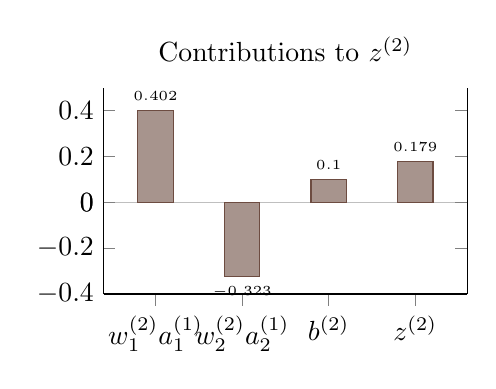
\begin{tikzpicture}
\begin{axis}[width=6.2cm,height=4.2cm,ybar,bar width=0.45cm,ymin=-0.4,ymax=0.5,xmin=0.4,xmax=4.6,xtick={1,2,3,4},xticklabels={$w^{(2)}_1a^{(1)}_1$,$w^{(2)}_2a^{(1)}_2$,$b^{(2)}$,$z^{(2)}$},nodes near coords,nodes near coords style={font=\fontsize{5.5}{6.5}\selectfont,/pgf/number format/.cd,fixed,precision=3},title={Contributions to $z^{(2)}$},axis x line*=bottom,extra y ticks={0},extra y tick style={grid=major}]
\addplot[fill=AccentCol!60,draw=AccentCol] coordinates{(1,0.4021) (2,-0.3228) (3,0.1) (4,0.1793)};
\end{axis}
\end{tikzpicture}}
\begin{wbox}\scriptsize Hidden unit 2 \emph{pulls the output down}: its positive activation meets a negative weight. Hold this thought --- it explains a sign in the backward pass.\end{wbox}
\end{columns}
\end{frame}

\begin{frame}{Forward Pass F5 --- Loss, and the Forward Summary}
\begin{columns}[T]
\column{0.50\textwidth}
\subhead{F5: binary cross-entropy}
Since $y=1$, the $(1-y)$ term vanishes:
{\small\[
L=-\ln(0.544701)=\hl{0.607519}
\]}
\begin{cbox}{Forward-pass results}
\centering\renewcommand{\arraystretch}{1.15}
\begin{tabular}{lr@{\qquad}lr}
\toprule
$z^{(1)}_1$&0.3000&$a^{(1)}_1$&0.574443\\
$z^{(1)}_2$&0.6000&$a^{(1)}_2$&0.645656\\
$z^{(2)}$&0.179282&$a^{(2)}=\hat y$&0.544701\\
\midrule
\multicolumn{4}{c}{Loss $L=0.607519$}\\
\bottomrule
\end{tabular}
\end{cbox}
\column{0.47\textwidth}
\begin{ibox}\scriptsize\textbf{Interpretation:} the network is barely better than a coin-flip (54.5\%) on a target it should call ``hostile''. The backward pass tells each parameter how to move to raise that probability.\end{ibox}
\begin{cbox}[ISSAnavy]{Save for the backward pass}
\begin{tl}
\item $x_1,x_2$ \quad (multiply into $\partial L/\partial w^{(1)}$)
\item $a^{(1)}_1,a^{(1)}_2$ \quad (multiply into $\partial L/\partial w^{(2)}$, and give $\sigma'$)
\item $a^{(2)}$ \quad (gives $\delta^{(2)}$)
\end{tl}
Frameworks such as PyTorch store exactly these \emph{activations} in memory during the forward pass.
\end{cbox}
\end{columns}
\end{frame}

%====================================================================
\sect{9. Backward Pass}
\begin{frame}{The Chain Rule as a Computational Graph}
\centering
\begin{tikzpicture}[node distance=1.45cm,every node/.append style={font=\small},
 lb/.style={font=\scriptsize,text=ISSAgrey},lr/.style={font=\scriptsize,text=ISSAred}]
\node[ndG,font=\small] (w) {$w^{(1)}_{11}$};
\node[ndA,font=\small,right=of w] (z1) {$z^{(1)}_1$};
\node[ndA,font=\small,right=of z1] (a1) {$a^{(1)}_1$};
\node[ndA,font=\small,right=of a1] (z2) {$z^{(2)}$};
\node[ndA,font=\small,right=of z2] (a2) {$a^{(2)}$};
\node[ndR,font=\small,right=of a2] (L) {$L$};
\draw[arr] (w)--node[lb,above]{$\times x_1$}(z1);
\draw[arr] (z1)--node[lb,above]{$\sigma(\cdot)$}(a1);
\draw[arr] (a1)--node[lb,above]{$\times w^{(2)}_1$}(z2);
\draw[arr] (z2)--node[lb,above]{$\sigma(\cdot)$}(a2);
\draw[arr] (a2)--node[lb,above]{BCE}(L);
\draw[arrA,draw=ISSAred,bend left=40] (L) to node[lr,below]{$\frac{\partial L}{\partial a^{(2)}}$} (a2);
\draw[arrA,draw=ISSAred,bend left=40] (a2) to node[lr,below]{$a^{(2)}(1-a^{(2)})$} (z2);
\draw[arrA,draw=ISSAred,bend left=40] (z2) to node[lr,below]{$w^{(2)}_1$} (a1);
\draw[arrA,draw=ISSAred,bend left=40] (a1) to node[lr,below]{$a^{(1)}_1(1-a^{(1)}_1)$} (z1);
\draw[arrA,draw=ISSAred,bend left=40] (z1) to node[lr,below]{$x_1$} (w);
\node[lb,anchor=east] at ([xshift=-0.15cm]w.west) {forward $\rightarrow$};
\node[lr,anchor=west] at ([xshift=0.15cm,yshift=-0.55cm]L.east) {$\leftarrow$ backward};
\end{tikzpicture}
\vspace{3pt}
\begin{fbx}{Chain rule along the path}
$\dfrac{\partial L}{\partial w^{(1)}_{11}}=\underbrace{\dfrac{\partial L}{\partial a^{(2)}}\dfrac{\partial a^{(2)}}{\partial z^{(2)}}}_{\delta^{(2)}}\;\dfrac{\partial z^{(2)}}{\partial a^{(1)}_1}\;\dfrac{\partial a^{(1)}_1}{\partial z^{(1)}_1}\;\dfrac{\partial z^{(1)}_1}{\partial w^{(1)}_{11}}=\underbrace{\delta^{(2)}\,w^{(2)}_1\,\sigma'(z^{(1)}_1)}_{\delta^{(1)}_1}\,x_1$
\end{fbx}
\begin{ibox}\scriptsize\textbf{Backpropagation = the chain rule + reuse.} Compute $\delta^{(2)}$ once, reuse it for every output-layer gradient; compute each $\delta^{(1)}_j$ once, reuse it for every weight entering unit $j$.\end{ibox}
\end{frame}

\begin{frame}{Backward Pass B1 --- Output Error Signal $\delta^{(2)}$}
\begin{columns}[T]
\column{0.58\textwidth}
\subhead{Two local derivatives}
{\small
\begin{align*}
\frac{\partial L}{\partial a^{(2)}}&=-\frac{y}{a^{(2)}}+\frac{1-y}{1-a^{(2)}}=\frac{a^{(2)}-y}{a^{(2)}\bigl(1-a^{(2)}\bigr)}\\[3pt]
\frac{\partial a^{(2)}}{\partial z^{(2)}}&=\sigma'(z^{(2)})=a^{(2)}\bigl(1-a^{(2)}\bigr)
\end{align*}}
\subhead{Multiply: the $a^{(2)}(1-a^{(2)})$ factors cancel}
{\small\[
\delta^{(2)}=\frac{\partial L}{\partial z^{(2)}}=a^{(2)}-y=0.544701-1=\red{-0.455299}
\]}
\column{0.39\textwidth}
\begin{rbox}\textbf{The sigmoid + BCE identity}\\[2pt]\scriptsize $\delta^{(2)}=\hat y-y$: \emph{prediction minus target}. No $\sigma'$ factor at the output, so the output layer never saturates its own gradient. This is why BCE, not squared error, is paired with a sigmoid output.\end{rbox}
\begin{wbox}\scriptsize With squared error $L=\tfrac12(\hat y-y)^2$ we would get $\delta^{(2)}=(\hat y-y)\,\hat y(1-\hat y)=-0.1129$ --- four times weaker here, and near zero when the network is confidently wrong.\end{wbox}
\end{columns}
\end{frame}

\begin{frame}{Backward Pass B2 --- Output-Layer Gradients}
\begin{columns}[T]
\column{0.58\textwidth}
Since $z^{(2)}=w^{(2)}_1a^{(1)}_1+w^{(2)}_2a^{(1)}_2+b^{(2)}$:\quad $\dfrac{\partial z^{(2)}}{\partial w^{(2)}_j}=a^{(1)}_j,\ \ \dfrac{\partial z^{(2)}}{\partial b^{(2)}}=1$
{\small
\begin{align*}
\frac{\partial L}{\partial w^{(2)}_1}&=\delta^{(2)}a^{(1)}_1=(-0.455299)(0.574443)=\red{-0.261543}\\[3pt]
\frac{\partial L}{\partial w^{(2)}_2}&=\delta^{(2)}a^{(1)}_2=(-0.455299)(0.645656)=\red{-0.293967}\\[3pt]
\frac{\partial L}{\partial b^{(2)}}&=\delta^{(2)}=\red{-0.455299}
\end{align*}}
\column{0.39\textwidth}
\begin{cbox}{Gradient = error $\times$ input}
Every weight gradient is \hl{(error signal at the receiving unit)} $\times$ \hl{(activation on the sending side)}. A bias has input 1, so its gradient is the error signal itself.
\end{cbox}
\begin{ibox}\scriptsize All three gradients are negative, so gradient \emph{descent} will \emph{increase} $w^{(2)}_1$, $w^{(2)}_2$ and $b^{(2)}$ --- each increase raises $z^{(2)}$ and pushes $\hat y$ toward 1.\end{ibox}
\end{columns}
\end{frame}

\begin{frame}{Backward Pass B3 \& B4 --- Error Signals at the Hidden Layer}
\begin{columns}[T]
\column{0.58\textwidth}
\subhead{B3: sigmoid slopes at the hidden units}
{\small
\begin{align*}
\sigma'(z^{(1)}_1)&=a^{(1)}_1(1-a^{(1)}_1)=(0.574443)(0.425557)=\hl{0.244458}\\
\sigma'(z^{(1)}_2)&=a^{(1)}_2(1-a^{(1)}_2)=(0.645656)(0.354344)=\hl{0.228784}
\end{align*}}
\subhead{B4: back-propagate \ $\delta^{(1)}_j=\delta^{(2)}\,w^{(2)}_j\,\sigma'(z^{(1)}_j)$}
{\small
\begin{align*}
\delta^{(1)}_1&=(-0.455299)(0.7)(0.244458)=\red{-0.077911}\\
\delta^{(1)}_2&=(-0.455299)(-0.5)(0.228784)=\red{0.052083}
\end{align*}}
\column{0.39\textwidth}
\begin{wbox}\scriptsize\textbf{Why is $\delta^{(1)}_2$ positive?} $w^{(2)}_2<0$, so raising $a^{(1)}_2$ \emph{lowers} $\hat y$ --- the wrong direction for a hostile target. The gradient tells unit 2 to quieten down.\end{wbox}
\begin{cbox}{Shrinking signal}
$|\delta^{(2)}|=0.455$ but $|\delta^{(1)}_j|\le0.078$: one weight ($<1$) and one $\sigma'$ ($\le0.25$) cut the signal about $6\times$. Ten such layers would cut it by $\sim\!10^{8}$.
\end{cbox}
\end{columns}
\end{frame}

\begin{frame}{Backward Pass B5 --- Hidden-Layer Gradients}
Rules:\quad $\dfrac{\partial L}{\partial w^{(1)}_{jk}}=\delta^{(1)}_j\,x_k,\qquad \dfrac{\partial L}{\partial b^{(1)}_j}=\delta^{(1)}_j$
\vspace{3pt}

\centering\small\renewcommand{\arraystretch}{1.35}
\begin{tabular}{l l r @{\qquad} l l r}
\toprule
& \textbf{Calculation} & \textbf{Gradient} & & \textbf{Calculation} & \textbf{Gradient}\\
\midrule
$\partial L/\partial w^{(1)}_{11}$ & $(-0.077911)(1.0)$ & $\red{-0.077911}$ & $\partial L/\partial w^{(1)}_{21}$ & $(0.052083)(1.0)$ & $\red{0.052083}$\\
$\partial L/\partial w^{(1)}_{12}$ & $(-0.077911)(0.5)$ & $\red{-0.038956}$ & $\partial L/\partial w^{(1)}_{22}$ & $(0.052083)(0.5)$ & $\red{0.026041}$\\
$\partial L/\partial b^{(1)}_{1}$ & $\delta^{(1)}_1$ & $\red{-0.077911}$ & $\partial L/\partial b^{(1)}_{2}$ & $\delta^{(1)}_2$ & $\red{0.052083}$\\
\bottomrule
\end{tabular}
\vspace{4pt}

\begin{fbx}{Matrix form: one outer product}
$\nabla_{W^{(1)}}L=\delta^{(1)}x^{\mathsf T}=\begin{pmatrix}-0.077911\\0.052083\end{pmatrix}\begin{pmatrix}1.0&0.5\end{pmatrix}=\begin{pmatrix}-0.077911&-0.038956\\0.052083&0.026041\end{pmatrix}$
\end{fbx}
\end{frame}

\begin{frame}{Backward-Flow Diagram}
\figc{5.2cm}{%
\begin{tikzpicture}[x=1cm,y=1cm,
 neu/.style={circle,draw=ISSAred,line width=0.6pt,minimum size=1.0cm,inner sep=0pt,align=center,font=\fontsize{6.5}{7.5}\selectfont},
 bar/.style={{Stealth[length=3.5pt]}-,line width=0.7pt,draw=ISSAred},
 wl/.style={font=\fontsize{5.8}{6.8}\selectfont,fill=ISSAvlight,inner sep=0.6pt,text=ISSAred}]
\node[neu,draw=ISSAgrn,fill=ISSAgrn!12] (x1) at (0,1.2) {$x_1$\\1.0};
\node[neu,draw=ISSAgrn,fill=ISSAgrn!12] (x2) at (0,-1.2) {$x_2$\\0.5};
\node[neu,fill=ISSAred!8] (h1) at (3.8,1.2) {$\delta^{(1)}_1$\\$-0.0779$};
\node[neu,fill=ISSAred!8] (h2) at (3.8,-1.2) {$\delta^{(1)}_2$\\$0.0521$};
\node[neu,fill=ISSAred!20] (o) at (7.6,0) {$\delta^{(2)}$\\$-0.4553$};
\node[ndR,font=\fontsize{6}{7}\selectfont] (L) at (9.8,0) {$L=0.6075$};
\draw[bar] (x1)--node[wl,above=0.5pt]{$-0.0779$}(h1);
\draw[bar] (x2)--node[wl,below=0.5pt]{$0.0260$}(h2);
\draw[bar] (x2)--node[wl,pos=0.72,sloped,above=0.5pt]{$-0.0390$}(h1);
\draw[bar] (x1)--node[wl,pos=0.72,sloped,below=0.5pt]{$0.0521$}(h2);
\draw[bar] (h1)--node[wl,above,sloped]{$-0.2615$}(o);
\draw[bar] (h2)--node[wl,below,sloped]{$-0.2940$}(o);
\draw[bar] (o)--node[wl,above]{$\hat y-y$}(L);
\end{tikzpicture}}
\begin{columns}[T]
\column{0.48\textwidth}
\begin{cbox}{How to read it}\scriptsize Nodes carry $\delta=\partial L/\partial z$. Edges carry $\partial L/\partial w$ for that connection = (node $\delta$ on the right) $\times$ (activation on the left).\end{cbox}
\column{0.48\textwidth}
\begin{ibox}\scriptsize Information now flows \emph{right to left}: the same graph, traversed backwards, delivers every gradient in one sweep.\end{ibox}
\end{columns}
\end{frame}

%====================================================================
\sect{10. Update \& Check}
\begin{frame}{All Gradients at a Glance}
\begin{columns}[T]
\column{0.52\textwidth}
\figc{5.4cm}{%
\begin{tikzpicture}
\begin{axis}[width=7.4cm,height=6cm,xbar,bar width=0.22cm,xmin=-0.62,xmax=0.2,ytick=data,
 yticklabels={$w^{(1)}_{11}$,$w^{(1)}_{12}$,$w^{(1)}_{21}$,$w^{(1)}_{22}$,$b^{(1)}_1$,$b^{(1)}_2$,$w^{(2)}_1$,$w^{(2)}_2$,$b^{(2)}$},
 y dir=reverse,xlabel={$\partial L/\partial\theta$},title={Gradient of every parameter},
 nodes near coords,nodes near coords style={font=\fontsize{5}{6}\selectfont,/pgf/number format/.cd,fixed,precision=4},
 extra x ticks={0},extra x tick style={grid=major,grid style={ISSAdark!60}}]
\addplot[fill=AccentCol!55,draw=AccentCol] coordinates{(-0.0779,1)(-0.0390,2)(0.0521,3)(0.0260,4)(-0.0779,5)(0.0521,6)(-0.2615,7)(-0.2940,8)(-0.4553,9)};
\end{axis}
\end{tikzpicture}}
\column{0.45\textwidth}
\begin{cbox}{What the signs say}
\begin{tl}
\item \textbf{Negative} gradient $\Rightarrow$ descent \emph{increases} the parameter
\item \textbf{Positive} gradient $\Rightarrow$ descent \emph{decreases} the parameter
\item Hidden unit 1 (feeds $+0.7$): all its incoming weights grow
\item Hidden unit 2 (feeds $-0.5$): all its incoming weights shrink
\end{tl}
\end{cbox}
\begin{ibox}\scriptsize Output-layer gradients are 3--6$\times$ larger than hidden-layer ones: the output layer learns fastest at first.\end{ibox}
\end{columns}
\end{frame}

\begin{frame}{One Gradient-Descent Step ($\eta=0.5$, assumed) and a Sanity Check}
\begin{columns}[T]
\column{0.52\textwidth}
\begin{fbx}{Update rule}
$\theta\leftarrow\theta-\eta\,\dfrac{\partial L}{\partial\theta}$
\end{fbx}
{\small
\begin{align*}
W^{(1)}&\leftarrow\begin{pmatrix}0.438956&-0.180522\\0.273959&0.586979\end{pmatrix}\\[2pt]
b^{(1)}&\leftarrow(0.038956,\ -0.026041)\\
w^{(2)}&\leftarrow(0.830772,\ -0.353017)\\
b^{(2)}&\leftarrow0.327650
\end{align*}}
\begin{rbox}\scriptsize Re-run the forward pass: $\hat y$: $0.5447\to\mathbf{0.6455}$, \ $L$: $0.6075\to\mathbf{0.4377}$. The loss fell, so the gradients are right.\end{rbox}
\column{0.45\textwidth}
\figc{4.9cm}{%
\begin{tikzpicture}
\begin{axis}[width=6.6cm,height=5.3cm,xmin=0,xmax=30,ymin=0,ymax=0.65,grid=major,grid style={ISSAgrey!20},xlabel={gradient-descent step},ylabel={loss $L$},title={Repeating the step 30 times ($\eta=0.5$)}]
\addplot[AccentCol,line width=1pt,mark=*,mark size=0.8pt] coordinates{(0,0.6075) (1,0.4377) (2,0.3326) (3,0.2638) (4,0.2164) (5,0.1822) (6,0.1567) (7,0.1369) (8,0.1213) (9,0.1087) (10,0.0983) (11,0.0896) (12,0.0822) (13,0.0759) (14,0.0705) (15,0.0657) (16,0.0615) (17,0.0578) (18,0.0545) (19,0.0515) (20,0.0488) (21,0.0464) (22,0.0442) (23,0.0422) (24,0.0403) (25,0.0386) (26,0.0371) (27,0.0356) (28,0.0343) (29,0.0330) (30,0.0318)};
\addplot[only marks,mark=*,mark size=1.8pt,ISSAred] coordinates{(1,0.4377)};
\node[font=\fontsize{5.5}{6.5}\selectfont,text=ISSAred,anchor=west] at (axis cs:2,0.45) {after today's step};
\node[font=\fontsize{5.5}{6.5}\selectfont,text=ISSAdark,anchor=east] at (axis cs:29,0.1) {$\hat y=0.969$ after 30 steps};
\end{axis}
\end{tikzpicture}}
\end{columns}
\end{frame}

\begin{frame}{Common Mistakes When Computing Backpropagation by Hand}
\begin{columns}[T]
\column{0.49\textwidth}
\begin{wbox}\textbf{1. Forgetting $\sigma'$ at hidden units.}\ \scriptsize $\delta^{(1)}_j=\delta^{(2)}w^{(2)}_j$ alone is wrong; multiply by $a^{(1)}_j(1-a^{(1)}_j)$.\end{wbox}
\begin{wbox}\textbf{2. Adding $\sigma'$ at the output.}\ \scriptsize With BCE the output $\sigma'$ has already cancelled: $\delta^{(2)}=\hat y-y$, not $(\hat y-y)\sigma'(z^{(2)})$.\end{wbox}
\begin{wbox}\textbf{3. Swapping indices.}\ \scriptsize $w^{(1)}_{jk}$ goes \emph{to} unit $j$ \emph{from} input $k$; its gradient is $\delta^{(1)}_j x_k$, not $\delta^{(1)}_k x_j$.\end{wbox}
\column{0.49\textwidth}
\begin{wbox}\textbf{4. Using updated weights mid-pass.}\ \scriptsize Compute \emph{all} gradients with the old weights first, then update everything together.\end{wbox}
\begin{wbox}\textbf{5. Sign of the step.}\ \scriptsize Descent is $\theta-\eta\nabla L$. Adding the gradient climbs the loss.\end{wbox}
\begin{ibox}\scriptsize\textbf{Self-check habit:} after any hand calculation, re-run the forward pass with the updated weights. If $L$ did not fall (for a small $\eta$), there is an error.\end{ibox}
\end{columns}
\end{frame}

\sect{11. Summary}
\begin{frame}{Part 2 Summary --- The Four Equations of Backpropagation}
\begin{columns}[T]
\column{0.55\textwidth}
\begin{fbx}{Output error (sigmoid + BCE)}$\delta^{(2)}=a^{(2)}-y$\end{fbx}
\begin{fbx}{Hidden error}$\delta^{(1)}_j=\delta^{(2)}\,w^{(2)}_j\,\sigma'(z^{(1)}_j)$\end{fbx}
\begin{fbx}{Weight gradients}$\dfrac{\partial L}{\partial w^{(2)}_j}=\delta^{(2)}a^{(1)}_j,\qquad \dfrac{\partial L}{\partial w^{(1)}_{jk}}=\delta^{(1)}_jx_k$\end{fbx}
\begin{fbx}{Bias gradients}$\dfrac{\partial L}{\partial b^{(2)}}=\delta^{(2)},\qquad \dfrac{\partial L}{\partial b^{(1)}_j}=\delta^{(1)}_j$\end{fbx}
\column{0.42\textwidth}
\begin{cbox}{Quick check (answers in the reference text)}
\begin{te}
\item If $y$ were 0, what would $\delta^{(2)}$ be?
\item Which hidden unit's weights would grow if $w^{(2)}_2$ were $+0.5$?
\item Why is $|\partial L/\partial w^{(1)}_{12}|$ exactly half of $|\partial L/\partial w^{(1)}_{11}|$?
\item What is the largest possible value of $\sigma'(z)$, and why does it matter for deep networks?
\end{te}
\end{cbox}
\begin{rbox}\scriptsize Forward: $L=0.6075$ \quad Backward: 9 gradients \quad One step: $L=0.4377$\end{rbox}
\end{columns}
\end{frame}


\begin{frame}{Looking Ahead --- Lecture 7: Convolutional Neural Networks}
\begin{columns}[T]
\column{0.50\textwidth}
\subhead{From dense layers to networks that see}
\begin{tl}\item Why a dense layer is a poor fit for a $64\times64$ image\item Convolution, ReLU and max-pooling computed by hand on a $6\times6$ image\item Output size $\lfloor(n+2p-k)/s\rfloor+1$; padding, stride, channels\item Parameter counting for a full CNN\item LeNet $\to$ AlexNet $\to$ VGG $\to$ ResNet; transfer learning\item Failure modes: adversarial patches, decoys, distribution shift\end{tl}
\begin{ibox}\scriptsize\textbf{Assignment 6:} single-neuron boundaries and XOR + a ReLU hidden-layer forward pass + a full sigmoid forward and backward pass + one update and the vanishing-gradient argument; bonus: parameter counting and depth.\end{ibox}
\column{0.46\textwidth}
\begin{cbox}{Preview: SAR target recognition}\scriptsize A $64\times64$ SAR chip passes through three convolution--pooling blocks (32, 64, 128 filters), global average pooling and a 10-class softmax: \textbf{93,962} parameters in total --- fewer than a single dense layer on the flattened image would need.\end{cbox}
\begin{rbox}\scriptsize The CNN is trained by \emph{exactly} the backpropagation of today's Part~2. Only the layers are new.\end{rbox}
\end{columns}
\end{frame}
\end{document}
